\chapter{Background} \label{chap:bg}
In the previous chapter, we performed quantitative survivability analysis of NEMO

\section{Introduction}
\label{sec:intro-BG}
Mobile router plays the key role  in a mobile network and acts as the gateway for all its
nodes, connects them to the global Internet, forwarding signaling
validation.
%
Our work \emph{differs} from the previous works in a way that we
have used a cross layer approach to exploit the extension of

The rest of the chapter is organized as follows.
Our proposed seamless NEMO architecture is explained in
Section~\ref{sec:seamless_nemo}. 

\section{Seamless Handover Scheme for NEMO} \label{sec:seamless_nemo}
Original NEMO basic support protocol allowed only one
care-of-address registration per home address of a mobile router.

\begin{figure}
\begin{center}
  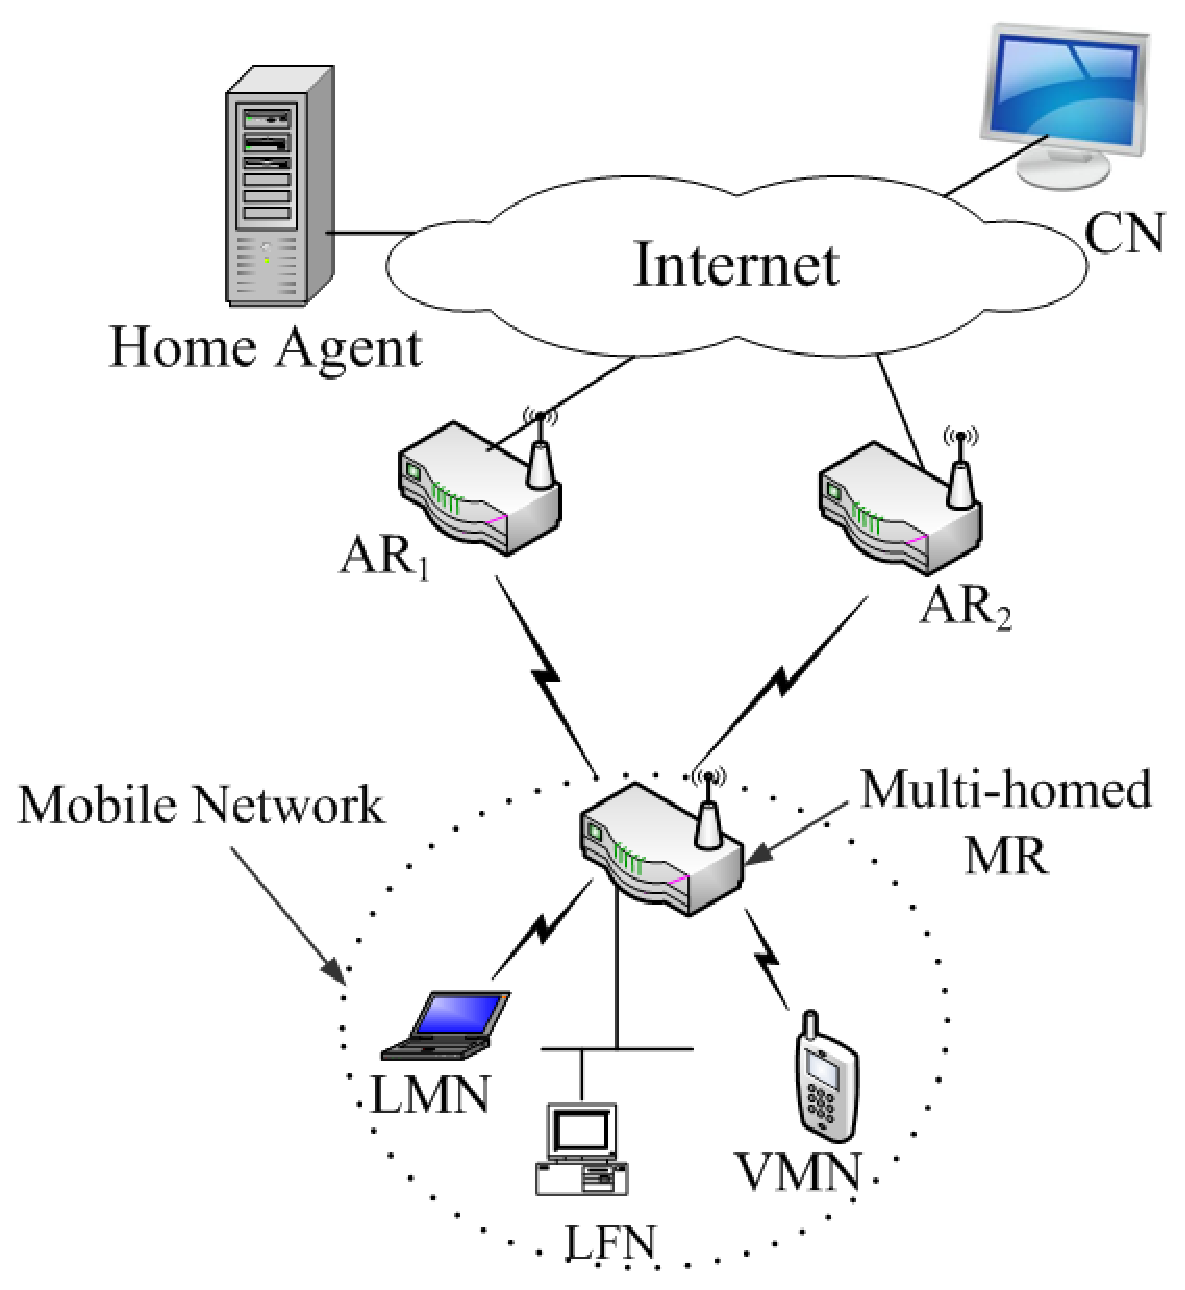
\includegraphics[width=3.2 in]{Back/M-NEMO}
   \caption{Architecture of multi-homed NEMO.}
   \label{fig:M-NEMO}
\end{center}
\end{figure}


\section{Experimental Setup}
\label{sec:testbed} For the performance evaluation of basic NEMO and
M-NEMO, we have used Linux-based experimental testbeds. The testbed

\begin{table}
\caption{Configuration of devices for M-NEMO testbed.}
\label{tab:mcoa_devices}
\begin{tabular}{|p{0.15in}|p{0.4in}|p{1.7in}|p{2.9 in}|}
%\hline No & Device Type & Software Configuration & Hardware Configuration\\
\hline \raisebox{-1.5 ex} {No} & Device Type & \raisebox{-1.5 ex} {Software Configuration} & \hspace{1.6 cm} \raisebox{-1.3 ex} {Hardware Configuration} \\
\hline 1 & MR & Ubuntu 8.04 Kernel 2.6.23 + NEPL & CPU: Intel Core 2 Duo, 2.20 GHz, 2 GB RAM, NIC: 802.11 based two Netgear MA111 \\
\hline 6 & APs & Channel 6 and Channel 11 & DLink WBR-1310 \\
\hline 7 & CN & Windows Vista  + FTP Server & CPU: Intel Core 2 Duo, 2.2 GHz, 2 GB RAM \\
\hline
\end{tabular}
\end{table}

%------------- Results -------------------
%------------- Results -------------------

\section{Results} \label{sec:results-MNEMO}
The experimental results are presented in this section. We measure
the throughput, Round Trip Time (RTT) and handoff latency by


\subsection{Throughput} The rate at which payload data are received
at any node is termed as its throughput. In our experiment, LFN
receives data traffic from CN. 

Fig.~\ref{fig:Thr-NEMO} shows the throughput at  LFN for NEMO BSP
tested during handoff between home network and foreign network. 

\begin{figure*}[bht]
\begin{minipage}[]{0.47\linewidth}
\centering
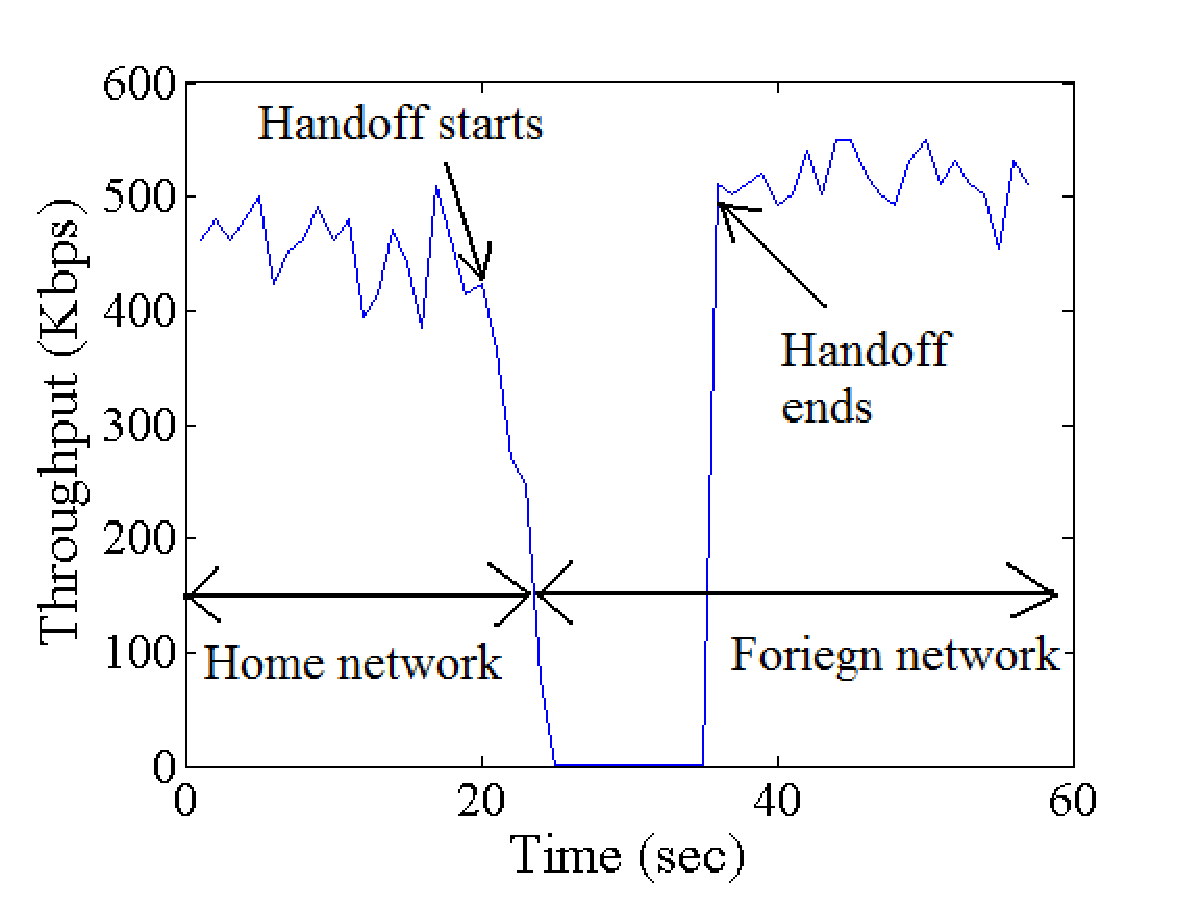
\includegraphics[width =3.0 in]{Back/Thr-NEMO}
\caption{Throughput at LFN for NEMO BSP.} \label{fig:Thr-NEMO}
\end{minipage}
\hspace{0.4cm}
%
\begin{minipage}[]{0.47\linewidth}
\centering
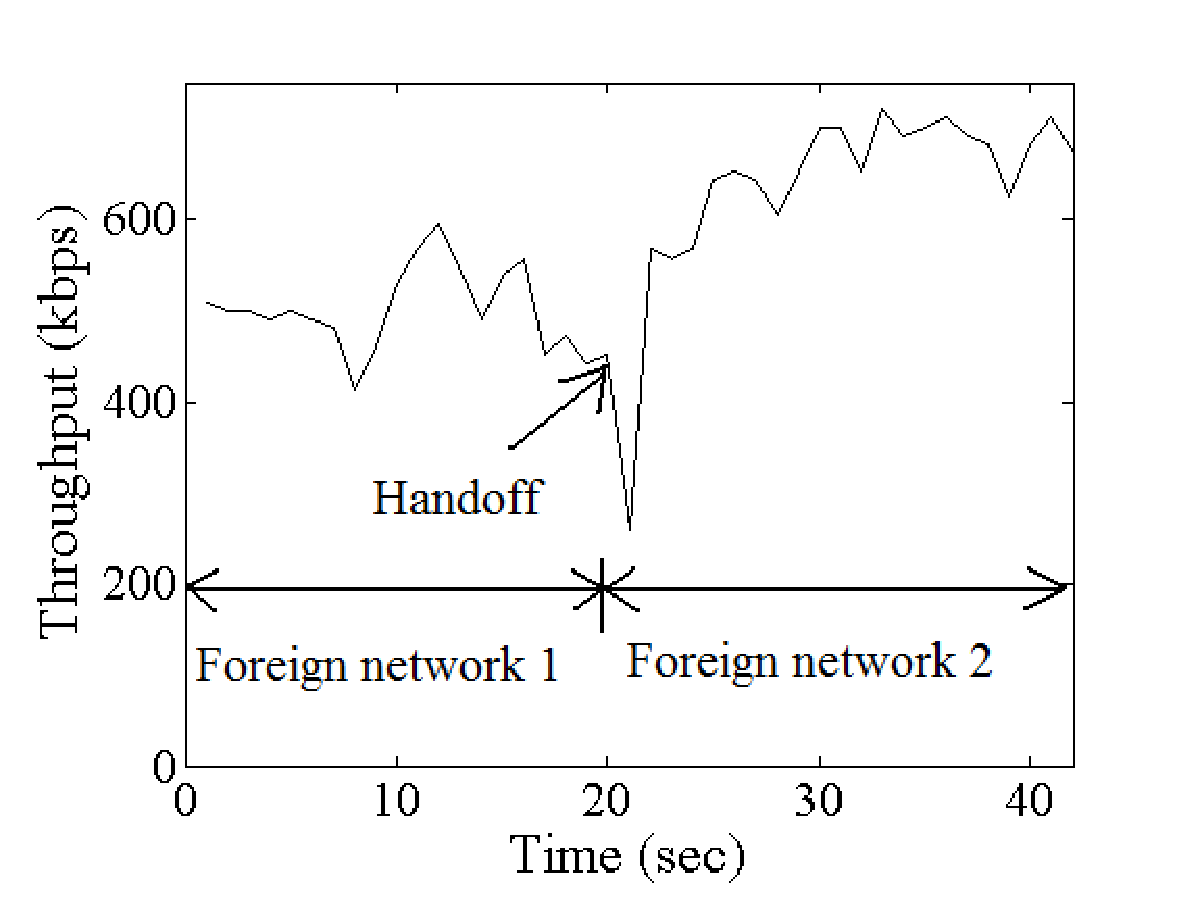
\includegraphics[width = 3.0 in]{Back/Thr-MNEMO}
\caption{Throughput at LFN for M-NEMO.} \label{fig:Thr-MNEMO}
\end{minipage}
%
\end{figure*}

Fig.~\ref{fig:Thr-MNEMO} shows the throughput at LFN for M-NEMO
testbed. Unlike NEMO BSP, the throughput in M-NEMO does not drop to
zero during the handoff period t = 20.073 sec to t = 20.148 sec.

\section{Summary}
\label{sec:summary-mnemo} In this chapter, we have proposed a
seamless handover scheme for NEMO exploiting the multihoming feature
of the mobile router. 

In the next chapter, we focus on the security issues and corresponding defense mechanisms of the mobility management protocols.
